\documentclass[etudiants]{support-iutrs}
\usepackage{pdfpages}
\usepackage{wrapfig}
\usepackage{graphicx}
\usepackage{subfig}

\infos{Benedick Steve, Meyblum Jean, Hagner Kevin}{P31}{T306AMAO}

\sujet{}
\titre{Ergonomie dans notre Projet T3}

\begin{document}
\header
\section{Petite introduction sur notre projet}

Notre projet a pour but la gestion informatique des emprunts et achats de bandes dessinées (BD) réalisés par un particulier.
Afin de gérer la saisie et l’enregistrement des bandes dessinées nous allons modifier une application déjà existante, Royal. 
Dans le but de faciliter l'ajout de BD dans Royal nous allons aussi mettre en place une application pour les téléphone Android, Royal\_Scanner.
Cette application permettra de scanner les codes barres afin de les envoyer au client PC Royal via un email.

Pour analyser l'ergonomie dans notre projet T3 nous travaillerons dans deux partie distinctes: 

-- La première traitera de l'ergonomie dans Royal.

-- La seconde partie traitera, quand à elle, de l'ergonomie dans Royal\_Scanner.

\section{Ergonomie dans Royal}
\paragraph{Interface graphique:}
Dans cette partie nous détaillerons l'interface graphique de la page principal de Royal mais les mêmes propriétés sont appliqués au autres pages de l'application. 

\subparagraph{Agencement de la fenêtre}
L'agencement de l'application Royal respecte assez bien les critères d'agencement vue en cour.

\begin{wrapfigure}[5]{l}[1cm]{5cm}
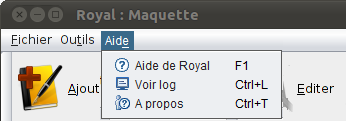
\includegraphics[width=5cm]{img/app_pc_maquette_menu.png}
\end{wrapfigure}

Tout d'abord nous retrouvons un menu regroupant les action secondaire de l'application tels que les préférences ou encore l'aide de Royal. 
Ce menu n'est pas surchargé (au maximum trois chois possibles) et rappel pour chaque action les raccourci clavier associé (ce qui est bon pour les utilisateurs expérimentés).

\begin{wrapfigure}[6]{r}[1cm]{8cm}
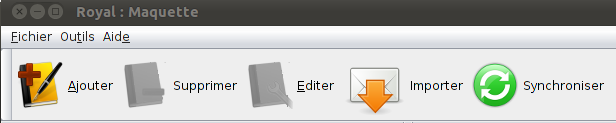
\includegraphics[width=8cm]{img/app_pc_maquette_btn.png}
\end{wrapfigure}

En-dessous nous retrouvons 5 boutons permettant d'effectuer les 5 principales actions de l'application. 
C'est 5 boutons sont accompagné d’icône ce qui les rends plus visible et facilite leurs compréhensions.
Ils sont placé à un endroit ou il sont très visible et facile d'accès ce qui est important vu qu'il s'agit des principales fonctionnalités de notre applications.

Dans la partie central de l'application nous retrouvons deux partie.

\begin{wrapfigure}[13]{l}[1cm]{7.5cm}
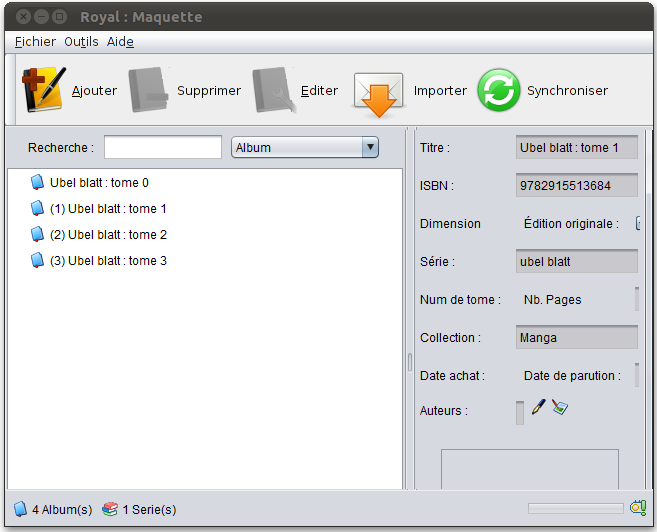
\includegraphics[width=7.7cm]{img/app_pc_maquette2.png}
\end{wrapfigure}
- A gauche: la partie affichant les différents Albums enregistrés dans Royal en fonction du critère d'affichage sélectionné. 

- A droite: la partie affichant les différentes informations sur l'album sélectionné.

Cette partie central propose bien une zone de sélection à gauche, et une zone de travail à droite.
Un problème d'ergonomie dans la partie gauche peu être observé lorsque la fenêtre est trop petite car certaine information n'ont pas la place pour être affiché mais le problème disparaît une fois la fenêtre agrandi. 
Pour corriger ce problème nous pouvons définir une largeur de fenêtre minimal afin d'assurer l’affichage de toute les informations. 

\begin{wrapfigure}[5]{r}[1cm]{6cm}
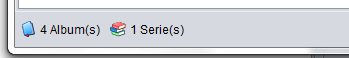
\includegraphics[width=6cm]{img/app_pc_maquette_bas.png}
\end{wrapfigure}

Enfin dans le bas de page nous retrouvons un récapitulatifs du nombre d'albums et de séries présents dans l'application.
Cette information étant optionnel ce n'est pas grave si elle est placé en-bas dans la fenêtre.

\subparagraph{Couleurs et police}
Les couleurs ainsi que les police choisie dans l'application Royal respecte assez bien les critère vue en cours.

L'application utilise des couleurs neutre et claire en fond. 
La partie regroupant les 5 boutons a un fond utilisant un autre gris que celui utilisé en fond de l'application se qui permet de la distingué rapidement. 
\begin{wrapfigure}[5]{l}[1cm]{6cm}
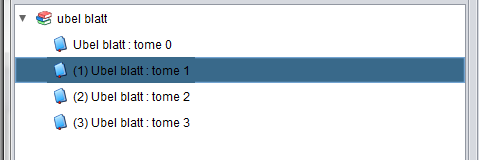
\includegraphics[width=6cm]{img/app_pc_maquette_elmt_selec.png}
\end{wrapfigure}

Pour la partie listant les différents albums qui utilise un fond blanc ce qui a nouveau permet de distingué cette partie. 
De même dans cette partie l'élément sélectionné aura un fond bleu se qui nous permet de le distingué des autres éléments.  

Pour le texte dans l'application une seul police est utilisé afin que l'application soit homogène. 
De même une seul couleur est utilisé, le noir car il contraste bien avec les fond clair utilisé dans l'application.  

\paragraph{Critères ergonomiques:}
\subparagraph{Compatibilité} Afin de s'intégrer à logique de l’utilisateur nous avons a vérifier la bonne compatibilité de notre application avec sa future utilisation.
  
\begin{wrapfigure}[5]{r}[1cm]{8cm}
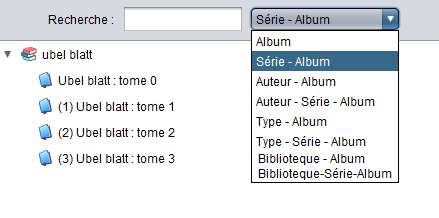
\includegraphics[width=8cm]{img/app_pc_maquette_lst.png}
\end{wrapfigure}\subparagraph{}
\subparagraph{}
Afin d'assurer cette compatibilité différents types d'affichage de la liste des albums seront proposé à l'utilisateur.
Ces différents types d'affichage se feront en fonctions de critères tels que l'auteur, le type ou encore la bibliothèque.


\subparagraph{Guidage et traitements des erreurs} 
Afin de facilité l'utilisation, l'utilisateur doit être guidé lors de l'utilisation du logiciel.

Afin de permettre ce guidage plusieurs éléments sont présent dans Royal.

\subparagraph{Dans la partie ajout/édition d'un album:}
\subparagraph{}

\begin{wrapfigure}[8]{l}[1cm]{8cm}
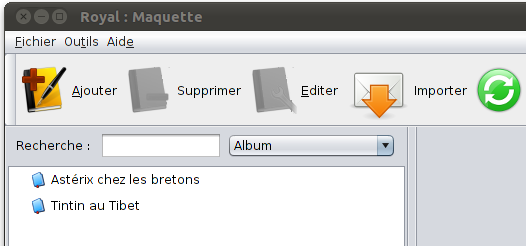
\includegraphics[width=8cm]{img/app_pc_maquette_btn_grise.png}
\end{wrapfigure}\subparagraph{}

Tout d'abord les boutons des actions ne pouvant être effectué sont grisé (par exemple la suppression ou l’édition d'un album sont grisé lorsque aucun album est sélectionné.

Le bouton supprimé demande aussi une validation de la suppression afin d'éviter la suppression d'album par erreur.
\clearpage

\begin{figure}[h!]
\begin{center}
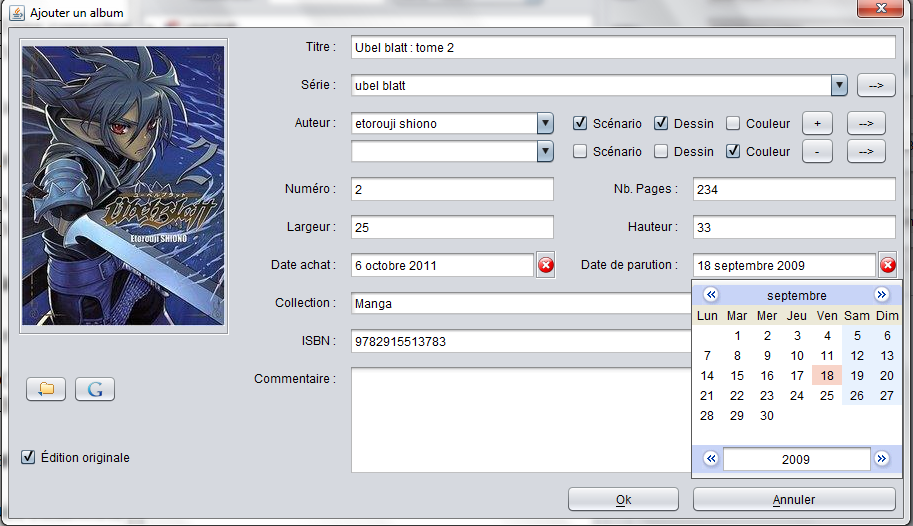
\includegraphics[width=12cm]{img/app_pc_maquette_ajout_album.png}
\end{center}
\end{figure}
Lors de l'ajout de date un calendrier est proposé à l'utilisateur afin qu’il sélectionne une date (ce mode de saisi d'une date permet aussi de limité les erreurs).

Lors de L'ajout d'auteur des radios bouton sont mis en place afin de permettre à l'utilisateur de choisir la fonction de l'auteur (tels que le dessin, le scénario...)

Afin d'éviter à l'utilisateur de saisir plusieurs fois la même information (par exemple l'auteur) il sera possible d'afficher une liste proposant les divers séries, auteurs, collections et bibliothèques déjà saisie dans l'application.

Afin d'éviter le surplus de champs dans la fenêtre des boutons on été mis en place afin de permettre d'ajouter plus d'information sur un élément (bouton ->) ou répéter un élément (bouton + pour les auteurs).

\begin{figure}[h!]
\begin{center}
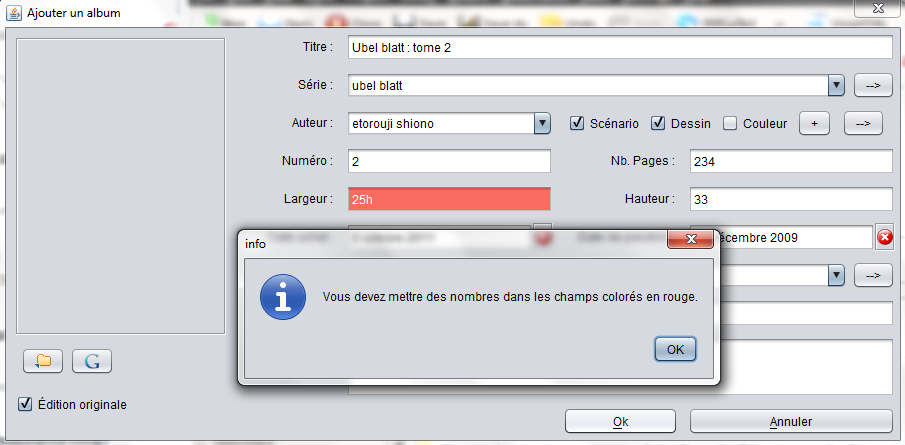
\includegraphics[width=12cm]{img/app_pc_maquette_erreur.png}
\end{center}
\end{figure}

Des vérifications sur la validité des informations ajouté dans les champs numérique tels que le numéro de tome on été ajouté. 
En cas de mauvaise saisie un message d'erreur apparaît afin d'inviter l'utilisateur de re-saisir l'information dans le bon format.
Les champs comportant des erreurs sont colorés en rouge afin d'être facilement trouvé par l'utilisateur. 

Cependant une vérification sur la validité de l'ISBN devra aussi être mis en place afin de vérifier que l'ISBN saisi soit d'un bon format (ISBN 10 ou ISBN 13).

De même le format (cm) devra être ajouter à la longueur et la largeur afin d'éviter toute confusion.    
\clearpage

\subparagraph{Partie importation albums}

\begin{wrapfigure}[8]{r}[1cm]{5cm}
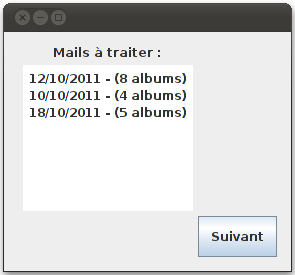
\includegraphics[width=5cm]{img/import_mail.png}
\end{wrapfigure}\subparagraph{}

Lors de l'importation d'albums via la boite mail l'application proposera à l'utilisateur de choisir le ou les email contenant des albums (l'application aura déjà filtré les email afin de ne proposé que les email provenant de l'application android ayant une syntaxe spécifique). 
Cette vérification automatique de la syntaxe des email permet d'éviter les erreurs en ne proposant a l’utilisateur que les email ayant la bonne syntaxe.
Cette vérification étant assez rapide il ne sera pas utile de mettre en place une barre de progression.
\subparagraph{}

\begin{wrapfigure}[7]{l}[1cm]{8cm}
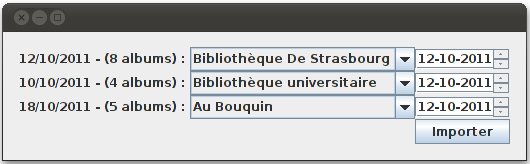
\includegraphics[width=8cm]{img/ajout_import.png}
\end{wrapfigure}
Une fois les email d'importation sélectionné une fenêtre permettant d'entrez le lieu et la date de retour de chaque lots d'emprunt apparaît (un email est égal a un lots).
Le champs de la bibliothèque de cette fenêtre à nouveau propose une liste avec les bibliothèque déjà saisi dans l’application afin d’éviter a l’utilisateur de les entrer a nouveau.
La date aussi sera a nouveau entré à l'aide d'un calendrier afin de facilité sa saisi et d'éviter les erreurs. 
Une vérification sur cette date sera aussi mis en place afin de vérifier que cette date n'est pas déjà passé.

Une fois les lieu et date validée un barre de progression affichera l’état de l'importation des lots. 
Une page récapitulatifs des informations ajouté sera affiché une fois l'importation terminé afin de détailler cette importation à l'utilisateur et lui montrer qu'elle a bien fonctionné.
 


\section{Ergonomie dans Royal\_Scanner}
\paragraph{Interface graphique:}
L'application Royal\_Scanner étant une application pour téléphone android il faudra adapter son interface graphique à un affichage mobile ainsi qu'à une utilisation tactile.

\subparagraph{Agencement de la fenêtre}
L’écran d'une téléphone mobile étant plus petit et moins large que celui d'un ordinateur il nous a fallu adapter certains critères d'agencement.

L'application devra veillez à ne pas surcharger l'écran afin que l'utilisation se fasse facilement.

  \begin{figure}[htbp]
  \begin{center}
    \leavevmode
    \subfloat[Page principal de l'application Royal\_Scanner]{%
		\label{}
		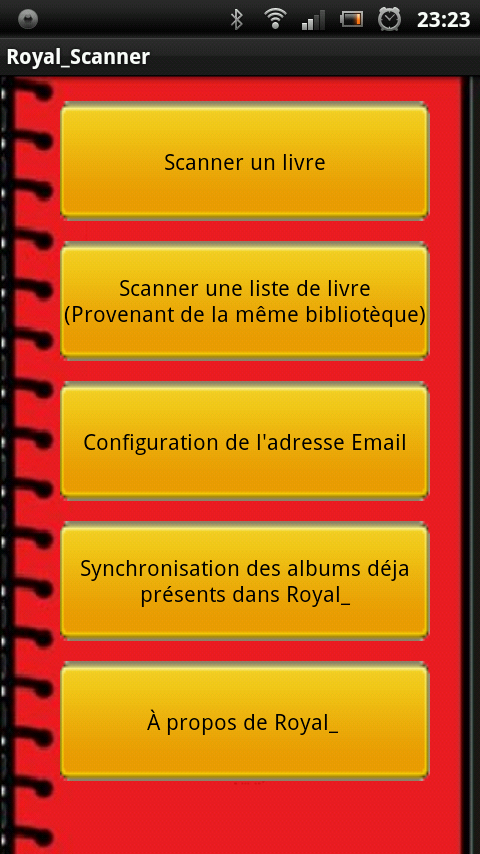
\includegraphics[height=6cm]{img/Menu_Royal_Scanner.png}}
    \hspace{4cm}
    \subfloat[Menu de l'application Royal\_Scanner]{%
		\label{}
		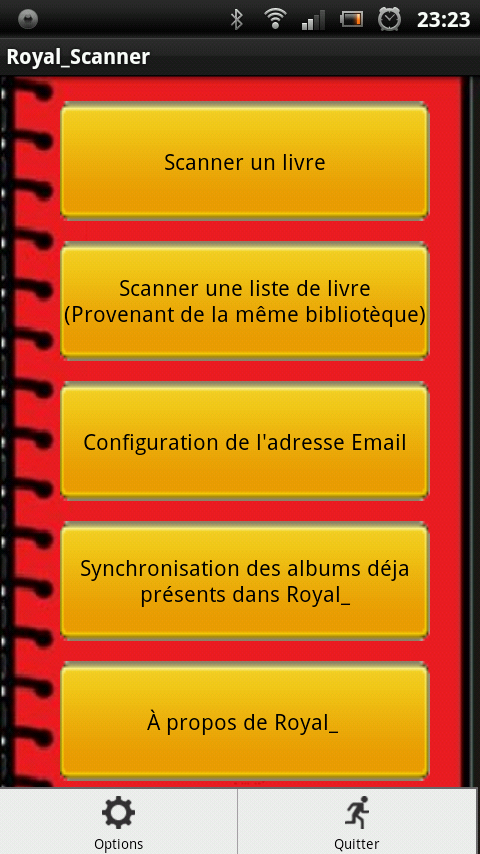
\includegraphics[height=6cm]{img/Menu_Royal_Scanner_option.png}}
  \end{center}
\end{figure}

Afin de proposer les principales action de l'applications mobile à l’utilisateur, une page principales regroupant les différentes actions dans des boutons lui sera proposé.
Afin de garantir leurs accessibilités ces boutons seront assez grand afin d'être adapter à une utilisation tactile. 

En cas de besoin un menu regroupant les fonctions secondaire de l'application sera mis en place.
Ce menu s'ouvrira lors de l’appuie de la touche menu du téléphone. 

  \begin{figure}[htbp]
  \begin{center}
    \leavevmode
    \subfloat[Configuration de l'adresse email dans Royal\_Scanner]{%
		\label{}
		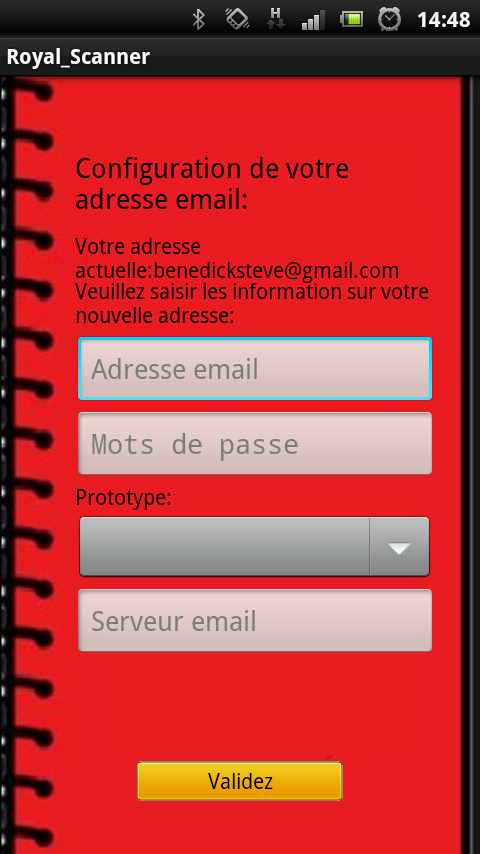
\includegraphics[height=6cm]{img/Configue_Email.png}}
    \hspace{4cm}
    \subfloat[Page d'envoi des ISBN scannés]{%
		\label{}
		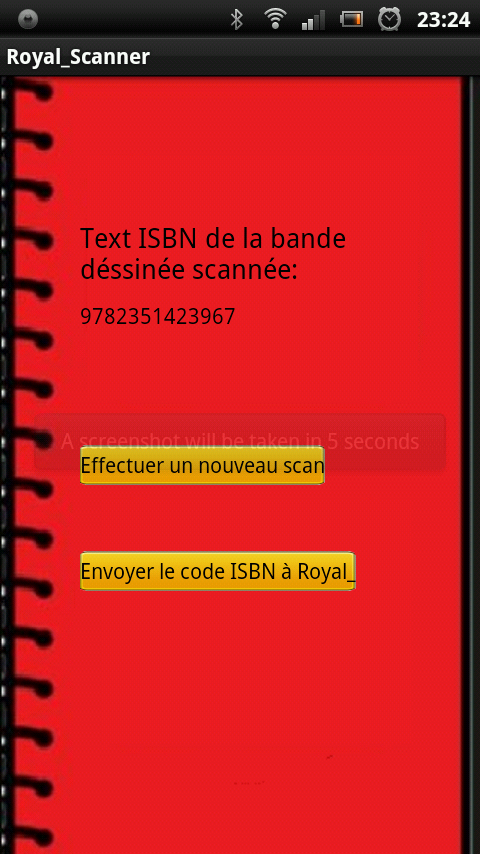
\includegraphics[height=6cm]{img/Scan_Multiple.png}}
  \end{center}
\end{figure}

Dans la page de configuration de l'adresse email le libellé des différents champs sera directement inclue dans le champs lui même.
Ce gain de place permet d'afficher l’intégralité de la page a l'écran ce que nous permet d'éviter l'oublie de champs par l'utilisateur.

Dans la seconde page, correspondant à la page s'affichant après le scan d'un code barre correspondant à un ISBN, le titre du livre sera ajouté à l'ISBN et affiché à l'utilisateur afin de lui montré le bon fonctionnement du scan. 

\subparagraph{Couleurs et police}
Les couleurs choisis dans l'application Royal\_Scanner bien que rappelant les couleurs du logo de Royal ne sont pas bonne et devront êtres modifiées.

Des couleurs plus neutres et claires tels que celles utilisé dans l'application PC seront utilisées pour le fond des différentes pages de l’application.

De même la couleurs des boutons sera modifié en une couleur plus neutre, seul le button selectionné aura une couleur plus vive afin d'etre distingué des autres boutons. 

Le style d'écriture de l'application Royal\_bouttonr dervrait quand à lui rester le même vu qu'il n'utilise qu'une seul police ce qui donne une certaine homogeneitée à l'application. 

\subparagraph{Guidage et traiements des erreurs}Les phases de saisie de l'utilisateur étants moin fréquentes que dans l'application PC nous n'aurrons qu'à les gerer dans la configuration de la boite mail.  

Tels que nous l'avont vu précedement lors de la configuration de la boite mail les libéllé de differents champs seront inclue dans le champs lui même.
 
De plus les champs seront configurés selon la valeurs qu'ils doivent retourner afin de proposer a l'utilisateur un clavier tactils optimiser pour la saisi de ces valeurs(par exemples pour le champs de l'adresse email un clavier proposant la touche '@' sera proposé).

Des verifications seront aussi effectué lors de la validation de la boite mail sur la validité des differents information contenu dans les champs.

En cas d'erreur un message d'erreur invitant l'utilisateur à ressaisir certaine information s'affichera en rouge à l'ecrans afin d'être vu par l'utilisateur. 

De même afin d'éviter l'apparition d'erreur dans la syntaxe de l'email envoyé à l'application PC nous ne passeront pas par une autres application pour envoyer l'email (car en passant par une autre aplication l'utilisateur peut modifier le contenu de l'email) nous géreront l'envoi de l'email dans l'application directement sans proposer l'édition de celui-ci par l'utilisateur. 

\end{document}
